\documentclass{article}

\usepackage{authblk}
\title{Supplementary Methods, Tables, and Figures}
\author[1]{Wancen Mu}
\author[2]{Eric Davis}
\author[3]{Stuart Lee}
\author[4]{Mikhail Dozmorov}
\author[2]{Douglas H. Phanstiel}
\author[1,2]{Michael I. Love \thanks{michaelisaiahlove@gmail.com}}
\affil[1]{Department of Biostatistics, and}
\affil[2]{Department of Genetics, University of North Carolina-Chapel Hill, NC 27599}
\affil[3]{Department of Econometrics and Business Statistics, Monash University, Clayton, Australia}
\affil[4]{Department of Biostatistics, Department of Pathology, Virginia Commonwealth University, Richmond, VA 23298, USA}

\date{\today}
\usepackage{graphicx}
\usepackage{graphics}
\usepackage{amsmath}
\usepackage{threeparttable}
\usepackage[top=1in,left=1in,right=1in,bottom=1in]{geometry}
\usepackage[usenames,dvipsnames,svgnames,table]{xcolor}
\usepackage{xspace}
% \usepackage{hyperref}
\usepackage[colorlinks=true,linkcolor=black,citecolor=blue,urlcolor=blue,]{hyperref}
\usepackage{natbib}
\usepackage{xcite}

% cross-ref with main paper
\usepackage{xr}
\makeatletter
\newcommand*{\addFileDependency}[1]{% argument=file name and extension
  \typeout{(#1)}
  \@addtofilelist{#1}
  \IfFileExists{#1}{}{\typeout{No file #1.}}
}
\makeatother
\newcommand*{\myexternaldocument}[1]{%
    \externaldocument{#1}%
    \addFileDependency{#1.tex}%
    \addFileDependency{#1.aux}%
}
\myexternaldocument{plain}


\usepackage[ruled,vlined,linesnumbered,noresetcount]{algorithm2e}
\newcommand\mycommfont[1]{\footnotesize\ttfamily\textcolor{blue}{#1}}
\SetCommentSty{mycommfont}
\usepackage{float}
\usepackage[section]{placeins}
\usepackage[capitalise,noabbrev]{cleveref}
\usepackage{stfloats}
\usepackage{bm}
\usepackage{booktabs}
\usepackage{diagbox} % for diag line in table
\usepackage{hyperref}
\usepackage{geometry}
\usepackage{bm}
\usepackage{amsfonts,amssymb} %font
\usepackage{amsthm}
\usepackage{booktabs}
\usepackage{subfigure}
\geometry{a4paper,scale=0.8}
\renewcommand{\thefigure}{S\arabic{figure}}
\renewcommand{\thetable}{S\arabic{table}}
\renewcommand{\thesubfigure}{\Alph{subfigure}}

\usepackage[utf8x]{inputenc} % deal with "-" not usually set up by the [utf8] option

\newcommand{\code}[1]{\texttt{#1}}
\newcommand{\bootranges}{\emph{bootRanges}\xspace}
\newcommand{\nullranges}{\emph{nullRanges}\xspace}
\newcommand{\granges}{\texttt{GRanges}\xspace}
\newcommand{\plyranges}{\emph{plyranges}\xspace}
\newcommand{\mike}[1]{\textcolor{red}{[Mike: #1]}}
\newcommand{\wancen}[1]{\textcolor{purple}{[wancen: #1]}}


\usepackage{listings}
\lstset{numbers=left, %设置行号位置
        numberstyle=\tiny, %设置行号大小
        keywordstyle=\color{blue}, %设置关键字颜色
        commentstyle=\color[cmyk]{1,0,1,0}, %设置注释颜色
        frame=single, %设置边框格式
        escapeinside=``, %逃逸字符(1左面的键),用于显示中文
        %breaklines, %自动折行
        extendedchars=false, %解决代码跨页时,章节标题,页眉等汉字不显示的问题
        xleftmargin=1em,xrightmargin=1em, aboveskip=1em, %设置边距
        tabsize=4, %设置tab空格数
        showspaces=false %不显示空格
       }
\usepackage{xcolor}

% \geometry{a4paper,left=2cm,right=2cm,top=1cm,bottom=1cm}

\begin{document}

\maketitle

\section{Supplementary Methods}\label{sec:suppmethods}

\subsection{Previous methods}
In order to generate background data sets for null hypothesis testing of association analysis, there are two ways to formulate.  
One method for generating background genomic features sets is to sample from a larger experimental pool or database, like 
LOLA \citep{sheffield2016lola} using Fisher's exact test, and Poly-Enrich \citep{lee2020poly} using likelihood ratio test based on negative binomial likelihood. 
Another method is to permute or shuffle the genomic ranges given random start sites to existing features, possibly considering an exclusion list of regions where features should not be located, like 
bedtools \citep{quinlan2010bedtools}, ChIP-Enrich \citep{welch2014chip},
GenometriCorr \citep{GenometriCorrfavorov2012}, GAT additionally allowing controlling for GC content \citep{GAT_2013}, and one of strategies of regioneR implement a circular randomization to preserve inter-feature distance \citep{gel2016regioner}.

\subsection{Segmentation formulation}
From annotation databases generated from Ensembl, we can obtain a sequence of gene density count per million base $\{X_1,...,X_n\}$ positioned linearly. We assume there exist integers $\bm{\tau}=\bm{\tau^{(n)}}=(\tau_0,...,\tau_U)$, where $0=\tau_0 < \tau_1 < ... <\tau_U = n$, such that the collections of variables, ${\bm{X}_{\tau_i},...,\bm{X}_{\tau_i+1}}$, are separately stationary for each $i=0,...,U-1$. We let $n_i=\tau_i-\tau_{i-1}$ be the length of the \textit{i}th region. Hence, we introduce the mapping $$\pi:\{1,...,n\}\rightarrow\{(i,j):1\leq i \leq U,1\leq j \leq n_i\}$$ which relates the original sequence $\{X_1,...,X_n\}$ to the segmentation sequence $\{X_{ij}:1\leq i \leq U,1\leq j \leq n_i\}$\\

\subsection{ChromHMM annotations for Roadmap Epigenomics}
\wancen{Should we talk about what is HMM and CBS?}
Data were downloaded from \url{https://egg2.wustl.edu/roadmap/web_portal/} which include 15 small states and summeraize them into 3 big categories: low density("E9","E13","E14","E15"), middle density("E10","E11","E12"), high density("E1-E8"). \wancen{XX pieces left after merging states and mean width is }

\subsection{Shuffling}\label{sec:shuffle}
Genome shuffling was performed by random sample SNPs in acceptance region on Genome with probability proportional to SNPs count on each chromosome. The acceptance region exclude all ENCODE excludable regions plus telomere,centromere from UCSC and rCGH derived from \code{excluderanges} for hg38 \citep{excluderanges}.

\subsection{Segmentation and block length chosen}\label{sec:length}
On the issue of 
block length selection, we considered it in two ways. One is trying to find $L_b$ that has the minimum value of a pseudometric $d^*(v)=|\sqrt{\frac{L_{v-1}}{L_v}}IQR(\mathcal{L}_{L_v})-IQR(\mathcal{L}_{L_{v-1}})|$ where $\mathcal{L}_{L_v}$ is the statistic distribution at length $L_v$, $v=1,2,\cdots,V$, V is the number of candidate block length and $IQR(\mathcal{L})$ is the interquartile range of statistics distribution followed \citet{bickel2010subsampling}.
Second way was evaluating conserved spatial pattern that generated null sets have similar properties with original sets, eg. inter-feature distance. We used the Earth's Mover distance(EMD) to quantify the similarity between the distributions of a inter-feature distance in the original  and  null  dataset,  resulting  in  values  between  zero  (identical  dis-tributions)  to  one  (totally  disjoint  distributions). The Earth Mover's Distance (EMD) between two distributions is proportional to the minimum amount of work required to change one distribution into the other. $$EMD(y,y') = \frac{min_{F=(f_{ij}\in \mathcal{}F(y,y'))} WORK(F,y,y')}{min(w_{\sum},u_{\sum})}$$ where y and y' is the histogram of original and null inter-feature distance with bin size = 0.3. Since the EMD always decreased as $L_b$ increased because more neighbouring features reserved, the right $L_b$ should be chosen so that longer length doesn’t improve much as well as it is much smaller than the $L_s$.

\subsection{Vector linear statistics and Gaussian approximation}
Suppose we are interested in region overlap which is defined as one feature $\bm{x}\ T_1, ..., T_\alpha$ with lengths $\tau_1,..., \tau_\alpha$, and the feature $\bm{y}\ S_1, ..., S_\beta$ with lengths $\rho_1, ..., \rho_\beta$, then the region overlap of feature $\bm{x}$ with feature $\bm{y}$ is defined as $Q \equiv  \frac{1}{\alpha}\sum_{t=1}^\alpha V_t$ where $V_t=1-\prod_{k\in (T_t+\theta)}(1-J_k)$ and $J_k=1$ if position k belongs to feature B and 0 otherwise. $\theta$ is the shift among feature $\bm{x}$ and $\bm{y'}$, such as 1kb when linking promoters to gene. This statistic $V_t$ is stationary except for end effects due to feature instances crossing segment boundaries. Here $\alpha$ can be derived as $\sum_{k=1}^nI_{k-1}(1-I_k)$ where $I_k=1$ if position k belongs to feature A and 0 otherwise. After we do the block bootstrap according to the segmentation region, we generate R new sets of null features $\bm{y'}$ and $R\times \frac{n}{L_b}$ blocks. Therefore, we can do both genome-wise or block-wise analysis based on the question being addressed. Either using $Q^{1'}, Q^{2'}, ..., Q^{R'}$ or $Q^{1'}, Q^{2'}, ..., Q^{R\times \frac{n}{L_b}'}$ to construct a normal distribution $\mathcal{Q'}$ according to the Central Limit Theorem. Notate, if block-wise analysis is preferred, the SD of bootstrap distribution should be scaled by $\sqrt{L_b}$.

Null hypothesis of no associations with 0.05 type I error:
$$Q\leq \mathcal{Q'}_{0.975}$$
So that the z score in \cref{fig:result} is calculated by $$z = \frac{\widehat{Q} - \widehat{Q^*}}{ se_R(\widehat{Q})}$$ where $\widehat{Q(.)^*} = \frac{\sum_{r=1}^R \widehat{Q^*(r)}}{R}$ is the sample mean of the $R$ replications and $se_R(\widehat{Q}) = \sqrt{\frac{\sum_{r=1}^R [\widehat{Q^*(r)}-\widehat{Q(.)^*}]^2}{R-1}}$.

% $$P_{H_0}[R_n\geq r_{n}]\approx 0.05$$

\subsection{Swaping algorithm}\label{sec:algorithm}


% \begin{algorithm}
% \SetNoFillComment
% \caption{Block bootstrap GRanges across chromosome} \label{alg:supp_unseg}
%   \KwData{Feature GRanges, Block length($L_b$), bootstrap times(R), type('permute' or 'bootstrap')}
% \KwResult{Bootstrapped distribution of test statistics}
% \While{r \leq R}{
% \textbf{rearranges block:} Generate consecutive tiling blocks with width = $L_b$ \tcp*[l]{where 'bait' blocks will be moved} \\
% \uIf{permutation}{
% \textbf{random block:} Sample blocks without replacement from \textbf{rearranges block} \\
% }\ElseIf{bootstrap}{ 
%          $n_b = \sum_{j=1}^{24} ceiling(L_{c} / L_b)$\\
%          \textbf{random block:} Generate $n_b$ blocks with replacement and probability weights proportional to $L_c$ \tcp*[l]{these blocks are the 'bait' for capturing features in $\bm{y}$}\\}
% Find overlap of random blocks and feature $\bm{y}$ \tcp*[l]{use the bait to sample features in $\bm{y}$}\\
% Swap the ranges in those bait blocks given the shift between random block and rearranges block} \\
% Bind bootranges object which has $r$ and $L_b$ as metadata columns $\gets$ plyranges.
% \end{algorithm}


\begin{algorithm}[H]
  \SetAlgoLined
  \KwData{Feature GRanges, Block length($L_b$), bootstrap times(R), type('permute' or 'bootstrap')}
    \KwResult{Bootstrapped distribution of test statistics}
  \While{$r \leq R$}{
    \textbf{rearranges block:} Generate consecutive tiling blocks with width = $L_b$ \tcp*[l]{where 'bait' blocks will be moved}
    \uIf{permutation}{
\textbf{random block:} Sample blocks without replacement from \textbf{rearranges block} 
}\ElseIf{bootstrap}{ 
         $n_b = \sum_{j=1}^{24} ceiling(L_{c} / L_b)$\\
         \textbf{random block:} Generate $n_b$ blocks with replacement and probability weights proportional to $L_c$ \tcp*[l]{these blocks are the 'bait' for capturing features in $\bm{y}$}
      }
Find overlap of random blocks and feature $\bm{y}$ \tcp*[l]{use the bait to sample features in $\bm{y}$}
Swap the ranges in those bait blocks given the shift between random block and rearranges block   
}
Bind bootranges object which has $r$ and $L_b$ as metadata columns $\gets$ plyranges
\caption{Block bootstrap GRanges across chromosome} \label{alg:supp_unseg}
\end{algorithm}



\begin{algorithm}
\SetNoFillComment
\caption{Segmented block bootstrap with proportional block length}\label{alg:framework}
  \KwData{Feature GRanges, Block length($L_b$), bootstrap times(R), segmentation GRanges }
\KwResult{Bootstrap distribution of test statistics}
\While{$r \leq R$}{
\For{each segmentation state $i$}{
\tcc{suppose $\alpha_i$ ranges in $\bm{y}$ of state $i$}
        $L_s^i = \sum_{j=1}^{\alpha_i} L_j$ \tcp*[l]{ $L_j$ is width of ranges}
         $L_b^i = L_b * L_s^i / L_c$ \tcp*[l]{block length of state $i$}
         $n_b^i = \sum_{j=1}^{\alpha_i} ceiling(L_{j} / L_b^i)$ \tcp*[l]{total \# of blocks}
         \textbf{random block:} Generate $n_b^i$ blocks start site with replacement and probability weights proportional to $L_j$ \tcp*[l]{these blocks are the 'bait' for capturing features in $\bm{y}$}
         \textbf{rearranges block:} Generate $n_b^i$ tiling blocks start site \tcp*[l]{where 'bait' blocks will be moved} 
         \textbf{Return:} random and rearranges block start and chromosome name
    }
Construct random blocks Granges and find overlap of random blocks and feature $\bm{y}$ \tcp*[l]{use the bait to sample features in $\bm{y}$}
Swap the ranges in those bait blocks given the shift between random block and rearranges block 
}
Bind bootranges object which has $r$ and $L_b$ as metadata columns $\gets$ plyranges
\end{algorithm}

\begin{algorithm}
\SetNoFillComment
\caption{Segmented block bootstrap with fixed block length across chromosome}\label{alg:supp_fixedlb}
  \KwData{Feature GRanges, Block length($L_b$), bootstrap times(R), segmentation GRanges }
\KwResult{Bootstrap distribution of test statistics}
\While{$r \leq R$}{
         $n_{j} = ceiling(L_{j} / L_b)$ \tcp*[l]{number of blocks within each ranges}
         $n_b = \sum_{j=1}^{\alpha} n_j$\tcp*[l]{suppose $\alpha$ ranges in feature $\bm{y}$}
         \textbf{random block:} Generate $n_b$ blocks start site with replacement and probability weights proportional to $L_j$ \tcp*[l]{these blocks are the 'bait' for capturing features in $\bm{y}$}
         \textbf{rearranges block:} Generate $n_b$ tiling blocks start site by order with width = $L_b$ \tcp*[l]{where 'bait' blocks will move to}
\For{each segmentation state $i$}{
         Identify random blocks chosen that are in state $i$ \\
         Identify rearranged blocks chosen that are in state $i$  \\
         \textbf{Return:} random block start, random block chromosome name, rearranges block start, rearranges block chromosome name
    }
Construct random blocks Granges, concatenate rearranges start and chromosome name vector\\
Find overlap of random blocks and feature $\bm{y}$ \tcp*[l]{use the bait to sample features in $\bm{y}$}
Swap the ranges in those bait blocks given the shift between random block and rearranges block 
}
Bind bootranges object which has $r$ and $L_b$ as metadata columns $\gets$ plyranges 
\end{algorithm}



% \input{dataprocess}\label{section:preprocessing}

\section{Supplementary Results} \label{sec:results}
\subsection{liver caQTL-GWAS colocalizations}
1872 SNP data was download from the NHGRI-EBI GWAS catalog \citep{gwascatalog} on September 22, 2021, extracted only single variant  associated with total cholesterol, and consensus peaks information of 20 samples were downloaded from GSE164870.
Then caQTL genomic coordinates were converted from hg19 to hg38 using \code{liftOver} to construct 221,606 peaks GRanges. Through the below code, variance of statistics and the z score in \cref{fig:result}a,b was derived.

\subsubsection{$L_b$ selection}
On the issue of 
block length selection, we considered it in two ways. One is trying to find $L_b$ that has the minimum value of a pseudometric $d^*(v)=|\sqrt{\frac{L_{v-1}}{L_v}}IQR(\mathcal{L}_{L_v})-IQR(\mathcal{L}_{L_{v-1}})|$ followed \citet{bickel2010subsampling}, where $\mathcal{L}_{L_v}$ is the statistic distribution at length $L_v$, $v=1,2,\cdots,V$ and $IQR(\mathcal{L})$ is the interquartile range. \cref{fig:suppfig}A showed $d^*$ were in common had smaller values when $L_b\in[300000,800000]$. Another way was evaluating conversing spatial distribution by assuming generated null sets have similar properties with original sets, eg. inter-feature distance. The Earth Mover's Distance (EMD) was used to access two distribution similarity because it is proportional to the minimum amount of work required to change one distribution into the other. Since the EMD always decreased as $L_b$ increased as more neighbouring features were reserved, the right $L_b$ should be chosen that a longer length won’t improve much as well as requesting $L_b$ is much smaller than the $L_s$. So [200000,600000] was shown to be  a good range by visualization and according to the Elbow Method of EMD(\cref{fig:suppfig}B-C). 

\begin{lstlisting}[language=R]
len <- do.call(c,lapply(boots, length))
Overlaps <-boots %>% join_overlap_left(y,maxgap=10e3) %>%
    group_by(iter) %>%
    summarize(rate = 1-sum(is.na(`y.id`))/len) %>%
    as.data.frame() %>% 
    select(rateOverlaps) %>% 
    summarise_all(funs(mean,var,IQR)) %>% 
    mutate(rate.z = abs(obs.mean-rate.mean)/sqrt(rate.var))

\end{lstlisting} 


\subsection{macrophage cell lines}\label{sec:splines}
Macrophage processed 24 RNA-seq samples and 145 ATAC-seq samples were loaded from \code{fluentGenomics}\citep{lee2020fluent}. They are measured after interferon gamma(IFNg) stimulation. Since the transcriptomic response to IFNg stimulation may be mediated through an increasing transcription factors bindings on nearby regions and ATAC-seq can captioned those regions' accessibility, we expect there is an enrichment of differentially accessible (DA) ATAC-seq peaks in the vicinity of differentially expressed (DE) genes. 

When performing block bootstrap with 5e5 block length on 100 times, we got $t_{99}=-108.1$ and p-value <.05. We could reject the null hypothesis and concluded that there was significant enrichment of DA peaks near DE genes by finding overlaps.

For fitting the generalized penalized splines, \code{gam} function in the \code{mgcv} package was used to fit the model, which used a penalized likelihood maximization, and generalized cross-validation is used to choose the optimal value for the smoothing parameter, $\lambda$. Then \code{tidymv} package was used to predict and extract the fitted value. 

\begin{lstlisting}[language=R]
boot_stats <- x %>% join_overlap_inner(`y'`) %>%
  group_by(id.x,iter) %>%
  summarize(count = n(), log2FC = max(log2FC)) %>%
  as.data.frame() %>%
  complete(`id.x`, iter, fill=list(count = 0)) %>%
  select(iter, count, logFC) %>%
  nest(-iter) %>%
  mutate(fit= map(data, ~gam(count ~ s(log2FC), data = .)),
         pred  = map(fit, ~predict_gam(model = .)),
         fitted = map(pred,~find_fit(data=.)))

\end{lstlisting} 

\subsection{Chromium Single Cell Multiome ATAC + Gene Expression assay}
Data were downloaded according to \citet{Vignette} instruction which includes genes and peaks in 10,032 cells. Cell type annotations have been done a priori by the 10x Genomics R\&D team. Then information on chromosome 1 to 22 were selected to construct gene and peak GRanges. Since the main goal is not to accurately find gene-promoter pairs but the realization, the following preprocess may not be the most suitable way. First, we aggregated cells within same cell types, to form ‘pseudobulks’ with 14 samples according to the metadata because psuedobulking provided smoother correlation statistics without loss of the information of interest. Next, remove all the features with 0 standard deviation. Then, log Compute counts per million (CPM) from \code{edgeR} was used to accounting for different library size.

Since genes' expression is most \textit{cis}-regulated by chromatin accessibility, there is a belief that two modalities would have significant high correlation. And extremely high expressed or low expressed genes would also have high or low accessibility in corresponding cell types. For the whole gene set, the mean correlation of genes and ATAC read counts was 0.33, while the subsampling correlation distribution in \cref{fig:suppfig} F had mean 0.007 across 1000 times block bootstrap. 5644 significant candidate
gene-promoter pairs were identified, among which 5591 genes had only
one pair, 25 genes had 2 pairs. 
% The most negative correlation gene TET3 has $\rho = -0.963$\cref{fig:suppfig}G outside the subsampling confidence interval [-0.85,0.78] and previous studies have assessed down-regulation TET3 are essential for B-cell development and tumorigenesis\citep{lio2019dysregulation}. Similarly, CD83\cref{fig:suppfig}H with $\rho = 0.992$ outside [-0.80, 0.68] was a well known myeloid markers\citep{li2019cd83}. 
So those significant pairs could provide important insights into perturb their promoters on chr2:74000098-74003475 and chr6:14116971-14139988 for future tumor treatment. 

The block below shows example code for running analysis
\begin{lstlisting}[language=R]
# split sparse count matrix into NumericList
x <- x_Granges %>%
  mutate(counts_X = NumericList(asplit(x.scaled, 1)))%>% sort()
y <- y_Granges %>%
  mutate(counts_y = NumericList(asplit(y.scaled, 1))) %>% sort()
# First standardize read counts for fast correlation computation
x$counts1 <- NumericList(lapply(x$counts_X,function(z)(z-mean(z))/sd(z)))
y$counts2 <- NumericList(lapply(y$counts_y,function(z)(z-mean(z))/sd(z)))

bootranges <- bootRanges(y,blockLength = 5e5, R=100)
  
# for standardized x and y:
correlation = function(x,y) 1/(length(x)-1) * sum(x*y)
## extract bootstrap summary statistics
boot_stats<-x %>% join_overlap_inner(boots, maxgap=1000) %>%
  mutate(rho = correlation(counts_x, counts_y)) %>%
  group_by(iter) %>%
  summarise(meanCor = mean(rho)) 
\end{lstlisting} 
 

\section{Supplementary Figures}
\begin{figure*}[t]
\centering
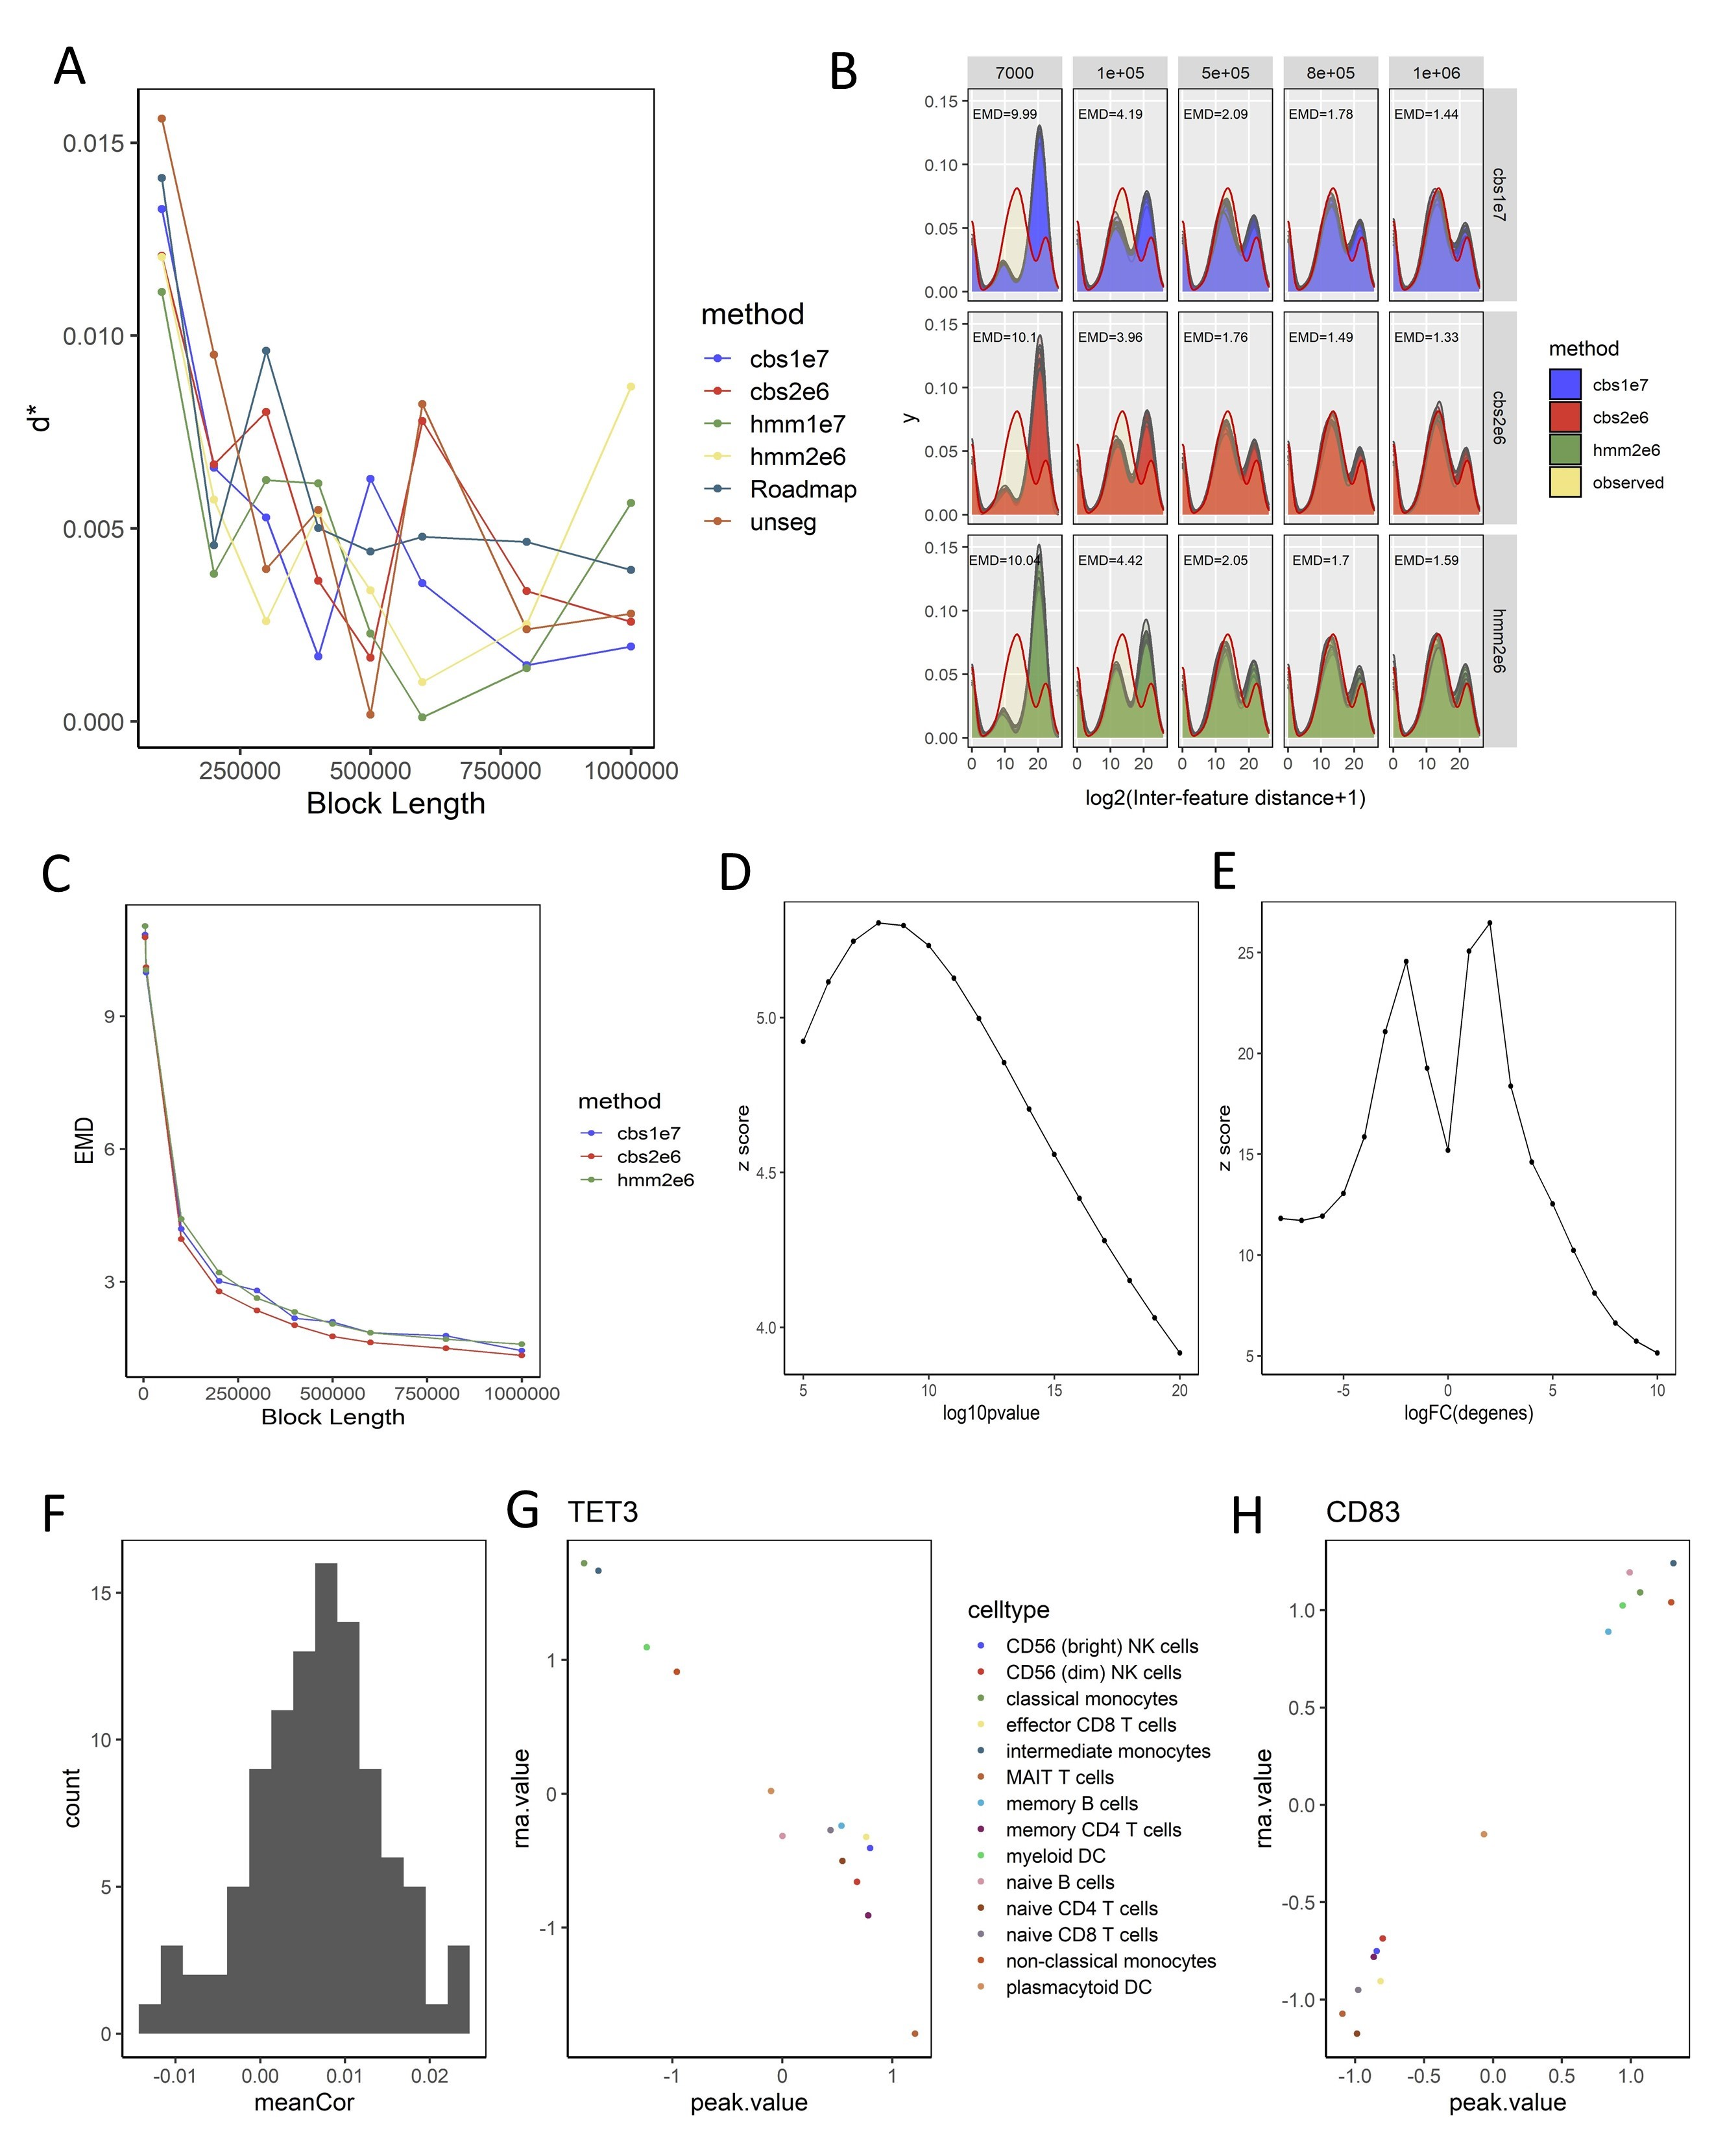
\includegraphics[scale=0.8]{Figures/sfig.jpg}
\caption{Bootstrapping parameter evaluation and enrichment analyses. A) A pseudometric $d^*$ over $L_b$, B) The null sets' log2(inter-feature distance+1) density plots generated by various block bootstrapped settings over observed feature set's distance. The more null sets' density plots overlapped with observsed features, the better conversing spatial distribution of original set captured. Medan EMD was shown as text in each panel. C) Median EMD over $L_b$ where EMD quantifies similarity between two distributions. D)\textit{z} score over -log10(pvalue) in ATAC-seq-GWAS analysis. \textit{z} score indicated the amount of standard deviations that observed fitted overlap rate away from 1000 times block bootstrap's fitted overlap rate. E) \textit{z} score over DE genes' logFC in macrophage enrichment analysis. \textit{z} score indicated the amount of standard deviations that observed fitted overlap count away from 1000 times block bootstrap's fitted overlap count. F)The mean correlation distribution of genes expression with 1000 times block bootstrapped ATAC's read counts. G) Gene TET3 read counts over peak chr2:74000098-74003475 read counts, colored by cell types. TET3 has the most negative correlation $\rho = −0.963$. H) Gene CD83 read counts over peak chr6:14116971-14139988 read counts, colored by cell types. The correlation of this gene-promoter pair is 0.992.} 
\label{fig:suppfig}
\end{figure*}

\bibliographystyle{natbib}
%\bibliographystyle{achemnat}
%\bibliographystyle{plainnat}
%\bibliographystyle{abbrv}
%\bibliographystyle{bioinformatics}
%
%\bibliographystyle{plain}
%
\bibliography{document}

\end{document}
